% ====== PAPER INFORMATION ======
% CONFERENCE NAME: 2026 International Conference on Software, Telecommunications and Computer Networks (SoftCOM)
% CONFERENCE PAPER: Characterizing Fairness Trade-offs in Multi-Client Adaptive Streaming Systems

% Number of Pages: 
% Regular: Not exceed 06 pages
% Format: IEEE-formatted double-column pages, including figures, tables, and references

% === Key Dates:
%   Original Paper Submission Deadline: May 20, 2026
%   Acceptance Notification: July 15, 2026
%   Conference Dates: September 22-24, 2026


\documentclass[conference,a4paper]{IEEEtran}
\IEEEoverridecommandlockouts
\usepackage{newtxtext}
% The preceding line is only needed to identify funding in the first footnote. If that is unneeded, please comment it out.
\usepackage{cite}
\usepackage{amsmath,amssymb,amsfonts}
\usepackage{algorithmic}
\usepackage{graphicx}
\usepackage{textcomp}
\usepackage{xcolor}
\usepackage{booktabs, multirow}
\usepackage{xcolor,colortbl}
\usepackage{soul}
\usepackage{changepage,threeparttable}


% NEW PERSONALIZED PACKAGES AND COMMANDS
% ##############################
\usepackage{booktabs} % For formal tables
\usepackage{xcolor,colortbl} % for cell colors
\usepackage{changepage,threeparttable} % for wide tables
\usepackage{float}
% \usepackage{hyperref} % For URL's references
\usepackage[bookmarks=false, hidelinks]{hyperref}
% \usepackage{nohyperref}
\usepackage{subcaption}
\usepackage{minted}
\usepackage[utf8]{inputenc}
\usepackage{cite}
\usepackage{longtable}
\usepackage{enumitem}
% \usepackage[subtle]{savetrees}

\renewcommand{\topfraction}{0.9}
\renewcommand{\bottomfraction}{0.8}
\renewcommand{\textfraction}{0.07}
\renewcommand{\floatpagefraction}{0.7}
\renewcommand{\dbltopfraction}{0.9}
\renewcommand{\dblfloatpagefraction}{0.8}
\renewcommand{\baselinestretch}{0.96}
\usepackage{etoolbox}
\patchcmd{\thebibliography}{\small}{\footnotesize}{}{}

\def\BibTeX{{\rm B\kern-.05em{\sc i\kern-.025em b}\kern-.08em
    T\kern-.1667em\lower.7ex\hbox{E}\kern-.125emX}}


% TEXT REVIEW COMMANDS
% ##############################
\usepackage{pifont} % http://ctan.org/pkg/pifont
\newcommand{\cmark}{\ding{51}}%
\newcommand{\xmark}{\ding{55}}%

% \newcommand{\rvi}[1]{{\color{blue}{#1}}} %included text - blue highlighting

\newcommand{\rvi}[1]{{\color{black}{#1}}} %included text - blue highlighting
\let\vi\rvi % Alias \vi to \rvi

\newcommand{\rvII}[1]{{\color{green}{#1}}} %included text second round revision
% \newcommand{\rvII}[1]{{\color{black}{#1}}} %included text

\newcommand{\rve}[1]{{\color{red}{#1}}} % excluded text




% TICKZ FIGURES
\usepackage{tikz}
\usetikzlibrary{arrows.meta,positioning,fit,calc}
\tikzset{
  >={Stealth[length=2.2mm,width=2.2mm]},
  box/.style={draw, rounded corners=2pt, thick, inner sep=6pt, align=center},
  title/.style={font=\bfseries\small},
  layer/.style={box, fill=gray!6, draw=gray!70},
  edgebox/.style={box, fill=purple!6, draw=purple!60},
  agentbox/.style={box, fill=orange!8, draw=orange!70!black},
  statebox/.style={box, fill=blue!6, draw=blue!55},
  envbox/.style={box, fill=teal!6, draw=teal!60!black},
  metricbox/.style={box, fill=teal!3, draw=teal!60!black},
  thinarrow/.style={-Stealth, very thick},
  dashedbox/.style={box, dashed, draw=gray!70, fill=gray!3},
}




% WATERMARK PERSONALIZATION
% \usepackage{draftwatermark}
% Configuração da marca d'água
% \SetWatermarkText{DRAFT} % Texto da marca d'água
% \SetWatermarkScale{1} % Tamanho da marca d'água
% \SetWatermarkColor[gray]{0.9} % Cor da marca d'água (0 = preto, 1 = branco)


\begin{document}

\title{Characterizing Fairness Trade-offs in Multi-Client Adaptive Streaming \\
% {\footnotesize \textsuperscript{*}Note: Sub-titles are not captured in Xplore and
% should not be used}
% \thanks{Identify applicable funding agency here. If none, delete this.}
}

\author{
\IEEEauthorblockN{1\textsuperscript{st} André Luiz de Moraes}
\IEEEauthorblockA{\textit{Computer Science} \\
\textit{\small Federal University of Santa Catarina (UFSC)} \\
Florianópolis, Brazil \\
chameoandre@gmail.com}
\and
\IEEEauthorblockN{2\textsuperscript{nd} Douglas D. J. de Macedo}
\IEEEauthorblockA{\textit{Dept. of Information Science (CIN)} \\
\textit{\small Federal University of Santa Catarina (UFSC)} \\
Florianópolis, Brazil \\
douglas.macedo@ufsc.br}

% 
% \and
% \IEEEauthorblockN{3\textsuperscript{rd} Antonio Brogi}
% \IEEEauthorblockA{\textit{Dept. of Computer Science} \\
% \textit{University of Pisa (UNIPI)} \\
% Pisa, Italy \\
% antonio.brogi@unipi.it}
% \and
% \IEEEauthorblockN{4\textsuperscript{th} Luiz Fernando Bittencourt}
% \IEEEauthorblockA{\textit{Institute of Computing} \\
% \textit{University of Campinas (UNICAMP)} \\
% Campinas, Brazil \\
% bittencourt@ic.unicamp.br}




% \and
% \IEEEauthorblockN{4\textsuperscript{th} Given Name Surname}
% \IEEEauthorblockA{\textit{dept. name of organization (of Aff.)} \\
% \textit{name of organization (of Aff.)}\\
% City, Country \\
% email address or ORCID}

% \and
% \IEEEauthorblockN{5\textsuperscript{th} Given Name Surname}
% \IEEEauthorblockA{\textit{dept. name of organization (of Aff.)} \\
% \textit{name of organization (of Aff.)}\\
% City, Country \\
% email address or ORCID}

% \and
% \IEEEauthorblockN{6\textsuperscript{th} Given Name Surname}
% \IEEEauthorblockA{\textit{dept. name of organization (of Aff.)} \\
% \textit{name of organization (of Aff.)}\\
% City, Country \\
% email address or ORCID}

}

\maketitle

% \begin{abstract}


% % ELEMENTS TO INCLUDE IN ABSTRACT

% % MAIN OBJECTIVE
% % Explore Fairness distribution in Adaptive Video streaming using a Reinforcement Learning Scheme exploring Edge computing capabilities.

% % Video Streaming growing and Lacks (Content providers dificulties, 
% % Importance of Machine Learning for Video Streaming Issues
% % Edge computing oportunities
% % Lack oportunities: Fairness between Bootleneck bandwidth clients
% % How different Fairness Measurement can benefit the choices of an Adaptive Streaming Session session.
% % Implementation objectives and structuration

% Video streaming represents the dominant share of today’s Internet traffic, making the efficiency and fairness of Adaptive Bitrate (ABR) algorithms increasingly critical. Conventional strategies largely focus on optimizing individual Quality of Experience (QoE) metrics such as startup delay, rebuffering, or video quality. However, these approaches frequently overlook fairness among users that compete for constrained and fluctuating network resources, especially in edge-assisted environments where bandwidth is highly variable.

% This work introduces a fairness-aware Reinforcement Learning (RL) approach for ABR decision-making, designed to leverage edge computing capabilities for timely and equitable resource allocation. We develop a multi-metric evaluation framework that incorporates both QoE and fairness dimensions. In addition to conventional QoE indicators (throughput, latency, rebuffering, and quality variations), we employ four complementary fairness metrics as decision variables: Temporal Fairness in QoE (TF-QoE), QoE Fairness Score (QFS), Bitrate Fairness Index (BFI), and Stability-Aware Fairness (SAF). 

% To validate our approach, we implemented a Docker-based simulation framework integrating Selenium for playback automation and Mahimahi for network emulation. Six ABR strategies were evaluated under controlled and identical network conditions: three heuristic-based baselines and three RL-based variants, including our proposed \textit{PENSIEVE-FAIRNESS} model. 

% Experimental results demonstrate that \textit{PENSIEVE-FAIRNESS} consistently outperforms heuristic and baseline RL methods across all fairness metrics, while maintaining or enhancing playback quality. These findings highlight the importance of fairness-driven learning for adaptive streaming and provide practical insights for the design of next-generation edge-assisted video delivery systems that are not only efficient, but also equitable in multi-user scenarios.

% \end{abstract}



\begin{abstract}
\vi{Ensuring fairness among users competing for shared network resources remains a critical challenge in multi-client adaptive video streaming. While modern adaptation strategies optimize individual Quality of Experience (QoE), they often overlook the complex trade-offs between different fairness dimensions and playback stability. This study presents an analytical characterization of these trade-offs by evaluating six diverse adaptation strategies, ranging from heuristic-based baselines to fairness-aware reinforcement learning, under identical, highly variable network conditions. We employ a multi-metric framework that jointly analyzes four complementary fairness indicators: Time-Fair QoE (TF-QoE), QoE Fairness Score (QFS), Bitrate Fairness Index (BFI), and Stability-Aware Fairness (SAF). By analyzing experimental data from a 10-client edge-assisted testbed replaying real-world 4G/3G traces, we reveal structural trade-offs between quality equity and adaptation stability. Our findings demonstrate that gains in bitrate fairness often come at the expense of increased quality switches for specific users, a trade-off that is significantly amplified under constrained network conditions. This work provides a rigorous observational baseline for the design of equitable streaming systems, highlighting that effective fairness evaluation must account for the interplay between resource distribution and temporal stability.}
\end{abstract}



% The increasing demand for adaptive video streaming presents significant challenges for content providers, particularly in ensuring high Quality of Experience (QoE) and fair bandwidth distribution among users with varying network conditions. Traditional Adaptive Bitrate (ABR) algorithms often face difficulties efficiently allocating resources under fluctuating network environments, leading to unfair bitrate allocation and degraded user experience, especially for bottlenecked clients. This work proposes a Reinforcement Learning (RL)-based approach that leverages Edge Computing capabilities to optimize QoE and fairness in adaptive streaming jointly. Our framework is deployed in a Docker-based infrastructure and tested using real-world network traces to simulate various network congestion levels. The experiments compare heuristic-based ABR methods with our RL-based approach, evaluating key QoE metrics such as average throughput, buffering time, and quality variations. Additionally, we assess fairness using Jain’s Fairness Index to measure how well the system distributes quality among users with different bandwidth constraints. Our results demonstrate that the RL-based approach significantly enhances fairness while improving overall QoE, particularly in highly variable and degraded network conditions ensuring smoother quality transitions and reduced playback disruptions. These findings highlight the potential of RL for advancing adaptive streaming strategies in Edge Computing environments, addressing key limitations of traditional ABR methods.

% \end{abstract}

\begin{IEEEkeywords}
\vi{Adaptive Bitrate (ABR) streaming, fairness trade-offs, edge computing, reinforcement learning, multi-metric evaluation, Quality of Experience (QoE).}
\end{IEEEkeywords}



\section{Introduction} \label{sec: Introduction}
    \vi{The rapid expansion of mobile data traffic has established video streaming as the primary consumer of Internet bandwidth, making the efficiency of video delivery systems a critical concern for content providers and network operators. To navigate highly variable cellular and edge networks, modern media players employ Adaptive Bitrate (ABR) algorithms, which dynamically adjust video quality representations based on real-time network conditions. While these algorithms are highly effective at optimizing individual Quality of Experience (QoE) parameters (such as minimizing buffering and maximizing playback resolution), they typically operate in a decentralized, client-centric manner.

    This client-centric design creates a major challenge in multi-user environments where concurrent clients compete for shared bottlenecks, such as edge nodes and cellular base stations. In these scenarios, independent adaptation loops lack coordination, leading to severe resource contention, high instability, and unfair quality distribution. While some recent studies propose coordinating resource allocation or introducing edge-assisted caching, the structural trade-offs between different dimensions of fairness and playback stability remain poorly understood. Conventional research evaluates fairness using aggregate indices like Jain's Fairness Index (JFI), which measure average resource distribution but completely mask the temporal dynamics and stability disparities that define the actual user experience. 

    To address this gap, this paper presents a multi-metric observational analysis of fairness trade-offs in edge-assisted multi-client streaming environments. We examine four distinct dimensions of fairness: temporal quality distribution (TF-QoE), overall distributional fairness (QFS), physical bitrate allocation (BFI), and adaptation stability (SAF). By evaluating six diverse ABR strategies under identical cellular network traces in a 10-client edge-assisted testbed, we expose a fundamental ``fairness-stability trade-off''. We demonstrate that algorithms optimizing strictly for resource or QoE equity often trigger severe playback instability for a subset of the client fleet, particularly during transient congestion windows. Our analysis clarifies that achieving holistic equity in multi-client systems requires a coordinated approach that goes beyond simple bitrate equalization.

    The main contributions of this work are: 
    \begin{itemize}[leftmargin=*, noitemsep, topsep=2pt, parsep=0pt]
        \item An analytical characterization of multi-dimensional fairness and stability trade-offs explicitly tailored for edge-assisted multi-client environments.
        \item The identification and detailed walk-through of the ``tactical panic'' (asymmetric downward switching under pressure) and ``recovery lag'' (persistent low-quality locks during bandwidth recovery) phenomena as primary drivers of temporal unfairness.
        \item Actionable design recommendations that outline how multi-metric observational findings can guide the development of next-generation edge-coordinated controllers, such as those utilizing reinforcement learning.
    \end{itemize}

    The remainder of the paper is organized as follows. Section \ref{sec:Related Works} reviews the related literature. Section \ref{sec:Background} provides the conceptual background and strict definitions of the evaluated fairness dimensions. Section \ref{sec:tradeoff_methodology} details the evaluation methodology. Section \ref{sec:results_discussion} presents the experimental results. Finally, Section \ref{sec:Conclusion and Future Work} concludes the paper.}

\section{Related Works \label{sec:Related Works}}
    \vi{While prior research established robust foundations for QoE optimization~\cite{mao2017neural,spiteri2020bola}, the interaction between multi-metric fairness and stability in multi-client scenarios remains insufficiently characterized. Previous works explored QoE fairness evaluation in edge layers~\cite{de2025joint,de2025fairness}, providing the experimental basis for this study. Heuristic strategies like FESTIVE~\cite{jiang2012improving} and BOLA~\cite{spiteri2020bola} improve stability but often lead to unfair resource distribution in multi-user scenarios. RL-based models like Pensieve~\cite{mao2017neural} and its extensions, such as Oboe~\cite{akhtar2018oboe} and HotDASH~\cite{hotdash2018}, prioritize individual QoE over equity.

    More recent fairness-aware metrics like QFS~\cite{hossfeld2018new} and BFI~\cite{li2023achieving} move beyond JFI but are rarely integrated into a structural analysis of adaptation trade-offs. Edge-assisted solutions like ARARAT~\cite{farahani2022ararat} and MEC-based policies~\cite{xiao2024qoe} investigate collaborative load balancing but still rely on aggregate indicators that mask temporal conflicts. 
    
    In broader network contexts, routing optimization in dynamic wireless environments, such as Flying Ad-Hoc Networks (FANETs) using metaheuristic algorithms~\cite{minocha2024optimized}, and stochastic assessments of communication network reliability under packet error constraints~\cite{Kumari2021Maintainable}, have also been proposed to address resource heterogeneity. However, these methods are not tailored to the application-level video quality dynamics of ABR. This study deconstructs these interactions by systematically analyzing how optimizing for different fairness dimensions presents trade-offs against playback stability under identical network variability, providing the necessary evidence to design next-generation, stability-aware fairness controllers.}

\section{Background Studies \label{sec:Background}}
    \vi{To establish a rigorous foundation for our trade-off analysis, we must define the core dimensions of adaptive video streaming, playback stability, and multi-metric fairness in multi-client systems.
    
    Adaptive Bitrate (ABR) streaming allows clients to dynamically select video representations based on network conditions and playback states. DASH-based implementations, such as DASH.js, typically employ heuristic rules based on throughput estimation or buffer occupancy to balance quality, rebuffering, and stability~\cite{jiang2012improving,yin2015control,spiteri2020bola}. While effective for independent users, these strategies lead to resource contention and unfair quality allocation in multi-client environments where bandwidth is shared. Data-driven approaches, particularly reinforcement learning (RL) \cite{mao2017neural}, have significantly improved individual QoE but often treat fairness as a secondary, post-hoc concern. 
    
    Standard indicators like Jain’s Fairness Index (JFI) \cite{jain1984quantitative} provide a limited view of equity, as they mask the temporal dynamics and recovery delays that define real-world user experience. Since fairness is inherently multi-dimensional, recent studies emphasize the necessity of complementary metrics that capture distributional equity, throughput allocation, and playback stability~\cite{hossfeld2017definition,hossfeld2018new,akhtar2020fairness}. 
    
    To address these limitations, we define four core concepts:
    \begin{itemize}[leftmargin=*, noitemsep, topsep=2pt, parsep=0pt]
        \item \textbf{Playback Stability:} Measures the frequency and magnitude of video representation changes (quality switches) during a streaming session. High instability (frequent switches) significantly degrades user QoE.
        \item \textbf{Distributional Equity:} Measures how evenly the composite Quality of Experience (QoE) is distributed among all concurrent clients sharing a network bottleneck, aggregated over the entire session.
        \item \textbf{Stability-Aware Fairness (SAF):} Captures whether the impact of adaptation instability is equitably distributed across the fleet. It quantifies whether some clients suffer disproportionately frequent quality switches compared to the average.
        \item \textbf{Quality Switch:} Defined as any transition in the selected video representation level between consecutive segments (e.g., from 1080p to 720p).
    \end{itemize}
    This multi-metric framework allows us to evaluate the joint trade-offs between resource distribution, QoE equity, and temporal stability in edge-assisted systems.}


    \begin{table*}[t]
        \centering
        \caption{Comparison of Related Works from a Fairness Evaluation Perspective}
        \label{tab:comparison_related_works}
        \scriptsize
        \begin{tabular}{|p{0.6cm}|p{2.9cm}|p{3.2cm}|p{4.6cm}|p{4.6cm}|}
        \hline
        \textbf{Work} & \textbf{Adaptation Strategy} & \textbf{Fairness Perspective} & \textbf{Evaluation Limitations} & \textbf{Evaluation Scope} \\
        \hline
        \cite{jiang2012improving} & Heuristic ABR (FESTIVE) & Implicit fairness via bandwidth sharing & No explicit fairness metrics; unstable under high heterogeneity & Early analysis of fairness side-effects in ABR \\
        
        \cite{spiteri2020bola} & Heuristic ABR (BOLA) & QoE stability-focused & Fairness not evaluated; single-client oriented & Robust buffer-based bitrate adaptation \\
        
        \cite{mao2017neural} & RL-based ABR (Pensieve) & QoE-centric optimization & Fairness not considered during decision-making & Learned bitrate adaptation for individual QoE \\
        
        \cite{akhtar2018oboe} & RL-based ABR (Oboe) & Efficiency and stability & No fairness evaluation & Automated tuning of ABR parameters \\
        
        \cite{hotdash2018} & Hybrid ABR (HotDASH) & Throughput efficiency & Ignores inter-client fairness & Content-aware bitrate adaptation \\
        
        \cite{hossfeld2018new} & Fairness metric proposal & QoE distribution fairness (QFS) & Metric-level evaluation only; no ABR integration & Definition and validation of QoE fairness metric \\
        
        \cite{li2023achieving} & Fairness metric proposal & Bitrate allocation fairness (BFI) & Single-metric fairness evaluation & Bitrate-based fairness assessment \\
        
        \cite{liu2022qoe-fairness} & Distributed bandwidth allocation & QoE-aware fairness & Focused on bandwidth allocation; limited metric diversity & Fairness-driven rate allocation at bottlenecks \\
        
        \cite{yuan2022muabr} & Multi-agent RL-based ABR & Fairness-aware coordination & Limited fairness metrics; scenario-specific evaluation & Coordinated bitrate decisions in multi-user scenarios \\
        
        \cite{farahani2022ararat} & Edge-assisted streaming & QoE improvement at the edge & Fairness treated implicitly or post-hoc & Edge-cloud collaboration for streaming \\
        
        \cite{xiao2024qoe} & MEC-based optimization & QoE fairness & Analytical modeling; limited experimental analysis & Fairness-aware resource allocation in MEC \\
        
        \cite{li2023edge-fair} & Edge-assisted ABR & Fairness via JFI & Single fairness metric; no trade-off analysis & Fairness-constrained ABR at the edge \\

        \vi{\cite{yau2025edge}} & \vi{Edge-centric heuristic} & \vi{Throughput-aware fairness} & \vi{Focus on estimation accuracy; ignores SAF} & \vi{Edge-based quality adaptation logic} \\

        \vi{\cite{huang2025balancing}} & \vi{RL-based ABR (Q2D3)} & \vi{QoE fairness vs preference} & \vi{Scenario-specific; lacks stability trade-off} & \vi{Cooperative edge server optimization} \\
        
        \hline\hline
        \textbf{This Work} & \textbf{Analytical Study} & \textbf{Multi-metric characterization} & \textbf{Observational perspective only} & \textbf{Characterizing fairness and stability trade-offs} \\
        \hline

        \end{tabular}
    \end{table*}


\section{Trade-off Analysis Methodology}
\label{sec:tradeoff_methodology}

    % ######################
    % SECTION: Trade-off Analysis Methodology
    %
    % OBJECTIVES OF THIS SECTION:
    % - Describe the methodological approach adopted to analyze fairness trade-offs in multi-client adaptive streaming.
    % - Define how multiple fairness and QoE-related metrics are jointly evaluated.
    % - Explain how experimental results are organized into comparable observation sets.
    % - Clarify that the analysis is observational and post-execution, without influencing adaptation decisions.
    % - Provide a reproducible framework for interpreting interactions between fairness dimensions and QoE stability.
    %
    % SCOPE AND POSITIONING:
    % - This section does not introduce new algorithms, control policies, or optimization mechanisms.
    % - All analyses are based on previously collected experimental data.
    The experimental data analyzed in this study are derived from controlled executions previously reported in related works~\cite{de2025joint,de2025fairness} and are reused exclusively for post-execution analysis. The analysis builds upon a validated experimental framework previously introduced by the authors~\cite{de2025joint,de2025fairness}, enabling a focused investigation of fairness trade-offs without confounding architectural variations. By maintaining consistent architectural assumptions across experiments, the analysis isolates the impact of adaptation behavior and network variability on fairness–stability trade-offs in multi-client environments.


    \begin{figure*}[t]
        \centering
        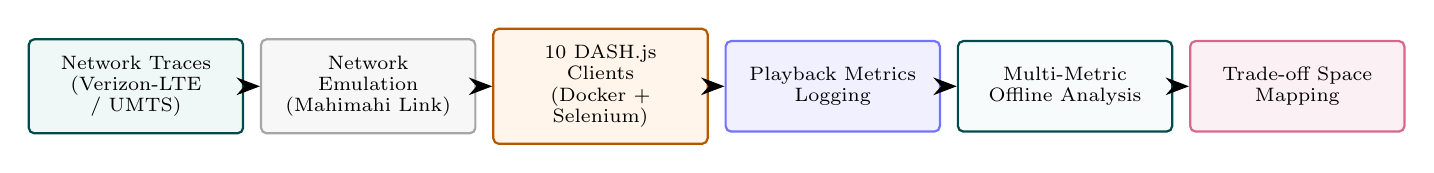
\begin{tikzpicture}[node distance=2mm, every node/.style={font=\scriptsize, text width=2.3cm, align=center, inner sep=2pt, minimum height=1.15cm}]
            \node[envbox] (traces) {Network Traces\\(Verizon-LTE / UMTS)};
            \node[layer, right=of traces] (mahimahi) {Network Emulation\\(Mahimahi Link)};
            \node[agentbox, right=of mahimahi] (docker) {10 DASH.js Clients\\(Docker + Selenium)};
            \node[statebox, right=of docker] (logs) {Playback Metrics\\Logging};
            \node[metricbox, right=of logs] (metrics) {Multi-Metric\\Offline Analysis};
            \node[edgebox, right=of metrics] (tradeoff) {Trade-off Space\\Mapping};

            \draw[thinarrow] (traces) -- (mahimahi);
            \draw[thinarrow] (mahimahi) -- (docker);
            \draw[thinarrow] (docker) -- (logs);
            \draw[thinarrow] (logs) -- (metrics);
            \draw[thinarrow] (metrics) -- (tradeoff);
        \end{tikzpicture}
        \caption{Experimental and analytical workflow for characterizing fairness--stability trade-offs in edge-assisted ABR streaming.}
        \label{fig:methodology_flowchart}
        \vspace{-0.2cm}
    \end{figure*}




    \subsection{Experimental Scenario}
    \label{subsec:experimantal-scenario}
        We focused on multi-metric fairness trade-offs and interaction effects, without modifying the underlying adaptation mechanisms. Table~\ref{tab:exp03-summary} summarizes the main characteristics of the experimental scenario to ensure clarity and self-containment.

        \begin{table}[t]
            \centering
            \caption{Summary of Experimental evaluation scenario.}
            \label{tab:exp03-summary}
            \vspace{-0.3cm}
            \scriptsize
            \vi{\begin{tabular}{p{2.6cm}|p{4.2cm}}
            \hline
            \textbf{Aspect} & \textbf{Description} \\
            \hline
            Scenario Type & Multi-client adaptive streaming under shared edge \\
            \hline
            Clients & 10 concurrent DASH clients in Docker containers \\
            \hline
            Streaming Engine & DASH.js player automated via Selenium \\
            \hline
            Network Traces & Verizon-LTE ($\mu \approx 20$ Mbps) and UMTS ($\mu \approx 2$ Mbps) \\
            \hline
            Video Content & Big Buck Bunny (6 levels: 360p--2160p) \\
            \hline
            Session & 120 seconds of playback per client \\
            \hline
            \end{tabular}}
        \end{table}



    \subsection{Overview of the Analytical Approach}
    
    The objective of the proposed methodology is to analyze trade-offs between multiple fairness metrics and Quality of Experience (QoE) indicators in multi-client adaptive streaming systems. Rather than optimizing a specific objective, the approach focuses on interpreting how different adaptation strategies influence fairness dimensions under shared network conditions. All analyses are performed offline using execution logs from controlled experimental scenarios, ensuring that adaptation decisions remain unaffected by the evaluation process.
    
    A structured analytical workflow is adopted in which executions are grouped into observation sets, complementary fairness metrics are computed independently, inter-metric correlations are evaluated, and adaptation strategies are mapped into a fairness--stability interaction space. This enables systematic identification of trade-off regions and competing optimization goals under identical network conditions.

    
    \subsection{Observation Sets and Experimental Grouping}
    
        Each observation set corresponds to a specific class of network behavior, such as relatively stable conditions or highly variable throughput patterns. By avoiding the aggregation of heterogeneous scenarios, the analysis prevents misleading conclusions caused by uncontrolled variability. Within each observation set, all ABR strategies are evaluated using the same set of clients, network traces, and execution parameters. This grouping enables direct comparison of fairness outcomes and QoE stability across adaptation strategies, highlighting how identical conditions can lead to different fairness profiles.
    
    \subsection{Multi-Metric Fairness Characterization}
        \vi{To move beyond single-index evaluation, we define four complementary fairness indicators that quantify distinct dimensions of resource distribution and playback stability. These equations form a unified framework spanning physical, perceptual, and temporal aspects of multi-user experience:

        \begin{itemize}[leftmargin=*, noitemsep, topsep=2pt, parsep=0pt]
            \item \textbf{TF-QoE (Time-Fair QoE):} Measures the relative deviation of client $i$'s composite QoE score ($Q_i$) from the session average ($\bar{Q}$):
            \vspace{-0.1cm}
            \begin{equation}
                TF\text{-}QoE_i = 1 - \frac{|Q_i - \bar{Q}|}{\bar{Q} + \epsilon}
                \label{eq:tf_qoe}
            \end{equation}
            \vspace{-0.1cm}
            where $Q_i$ is the composite QoE of client $i$, $\bar{Q} = \frac{1}{N}\sum_{j=1}^{N} Q_j$ is the mean composite QoE across all $N$ competing clients, and $\epsilon = 10^{-6}$ is a small regularization constant to prevent division by zero.

            \item \textbf{QFS (QoE Fairness Score):} Applies Jain's Fairness Index (JFI) \cite{jain1984quantitative} over the temporal average of composite QoE score samples ($\hat{Q}_i$) of all clients:
            \vspace{-0.1cm}
            \begin{equation}
                QFS = \frac{\left(\sum_{i=1}^{N} \hat{Q}_i\right)^2}{N \cdot \sum_{i=1}^{N} \hat{Q}_i^2}
                \label{eq:qfs}
            \end{equation}
            \vspace{-0.1cm}
            where $N$ represents the total number of concurrent clients sharing the bottleneck, and $\hat{Q}_i$ is the time-averaged composite QoE score for client $i$ during the streaming session.

            \item \textbf{BFI (Bitrate Fairness Index):} Evaluates fairness in physical resource allocation by applying JFI to the average numeric representation indices ($\bar{L}_i$):
            \vspace{-0.1cm}
            \begin{equation}
                BFI = \frac{\left(\sum_{i=1}^{N} \bar{L}_i\right)^2}{N \cdot \sum_{i=1}^{N} \bar{L}_i^2}
                \label{eq:bfi}
            \end{equation}
            \vspace{-0.1cm}
            where $\bar{L}_i$ is the average representation level index selected by client $i$, which ranges from 1 (lowest resolution, 360p) to 5 (highest resolution, 2160p).

            \item \textbf{SAF (Stability-Aware Fairness):} Characterizes the equity of adaptation stability across the fleet by comparing individual quality switch counts ($S_i$) to the average:
            \vspace{-0.1cm}
            \begin{equation}
                SAF_i = 1 - \frac{|S_i - \bar{S}|}{\bar{S} + \epsilon}
                \label{eq:saf}
            \end{equation}
            \vspace{-0.1cm}
            where $S_i$ is the total count of quality switches experienced by client $i$ during the session, and $\bar{S} = \frac{1}{N}\sum_{j=1}^{N} S_j$ is the average number of quality switches across all $N$ clients.
        \end{itemize}

        These four metrics are conceptually linked to capture the multi-dimensional nature of fairness. Specifically, $QFS$ evaluates overall distributional equity of perceived quality across the user fleet, but masks localized temporal deviations. To capture these individual experiences, $TF\text{-}QoE_i$ measures the localized temporal deviation of each client from the group mean. In contrast to these QoE-centric metrics, $BFI$ shifts the focus to the physical resource layer by assessing the fairness of raw bitrate representation levels. Finally, $SAF_i$ acts as an orthogonal stability-centric metric, evaluating whether the discomfort of adaptation oscillations (quality switches) is equitably shared among all competing clients. Together, these equations form a complete evaluation framework that bridges physical resource allocation ($BFI$), overall user satisfaction ($QFS$), individual temporal experiences ($TF\text{-}QoE_i$), and adaptation stability ($SAF_i$).}

    
\section{Results and Discussion}
\label{sec:results_discussion}
        \vi{This section presents the experimental findings and discusses the multi-metric fairness trade-offs under variable network conditions.}

        \begin{figure*}[t]
            \centering
            \begin{subfigure}[b]{0.49\textwidth}
                \centering
                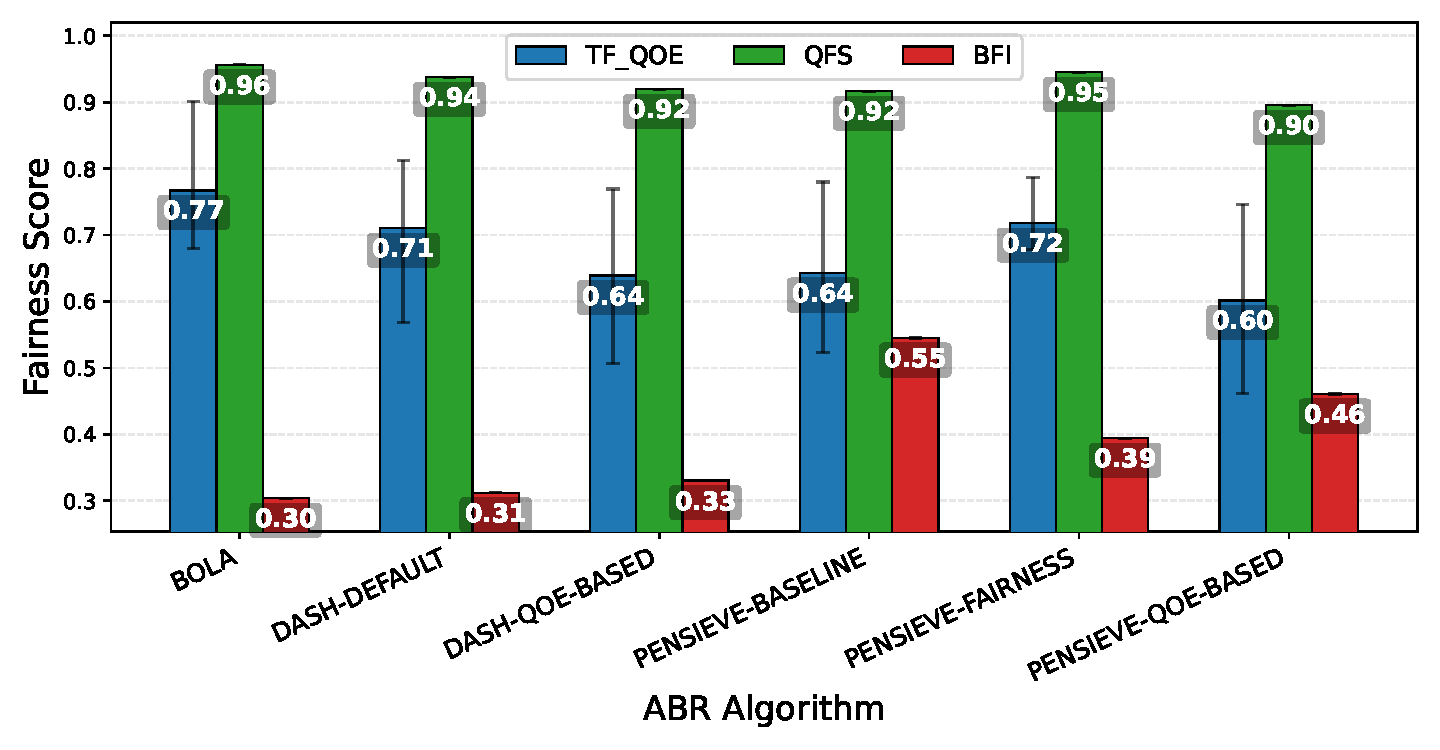
\includegraphics[width=0.98\linewidth,height=4.6cm,keepaspectratio=false]{images/p6-f1-fairness-metric-behavior-3.pdf}
                \caption{Fairness metric behavior (QFS, TF-QoE, BFI).}
                \label{fig:fairness_metrics_exp3}
            \end{subfigure}
            \hfill
            \begin{subfigure}[b]{0.49\textwidth}
                \centering
                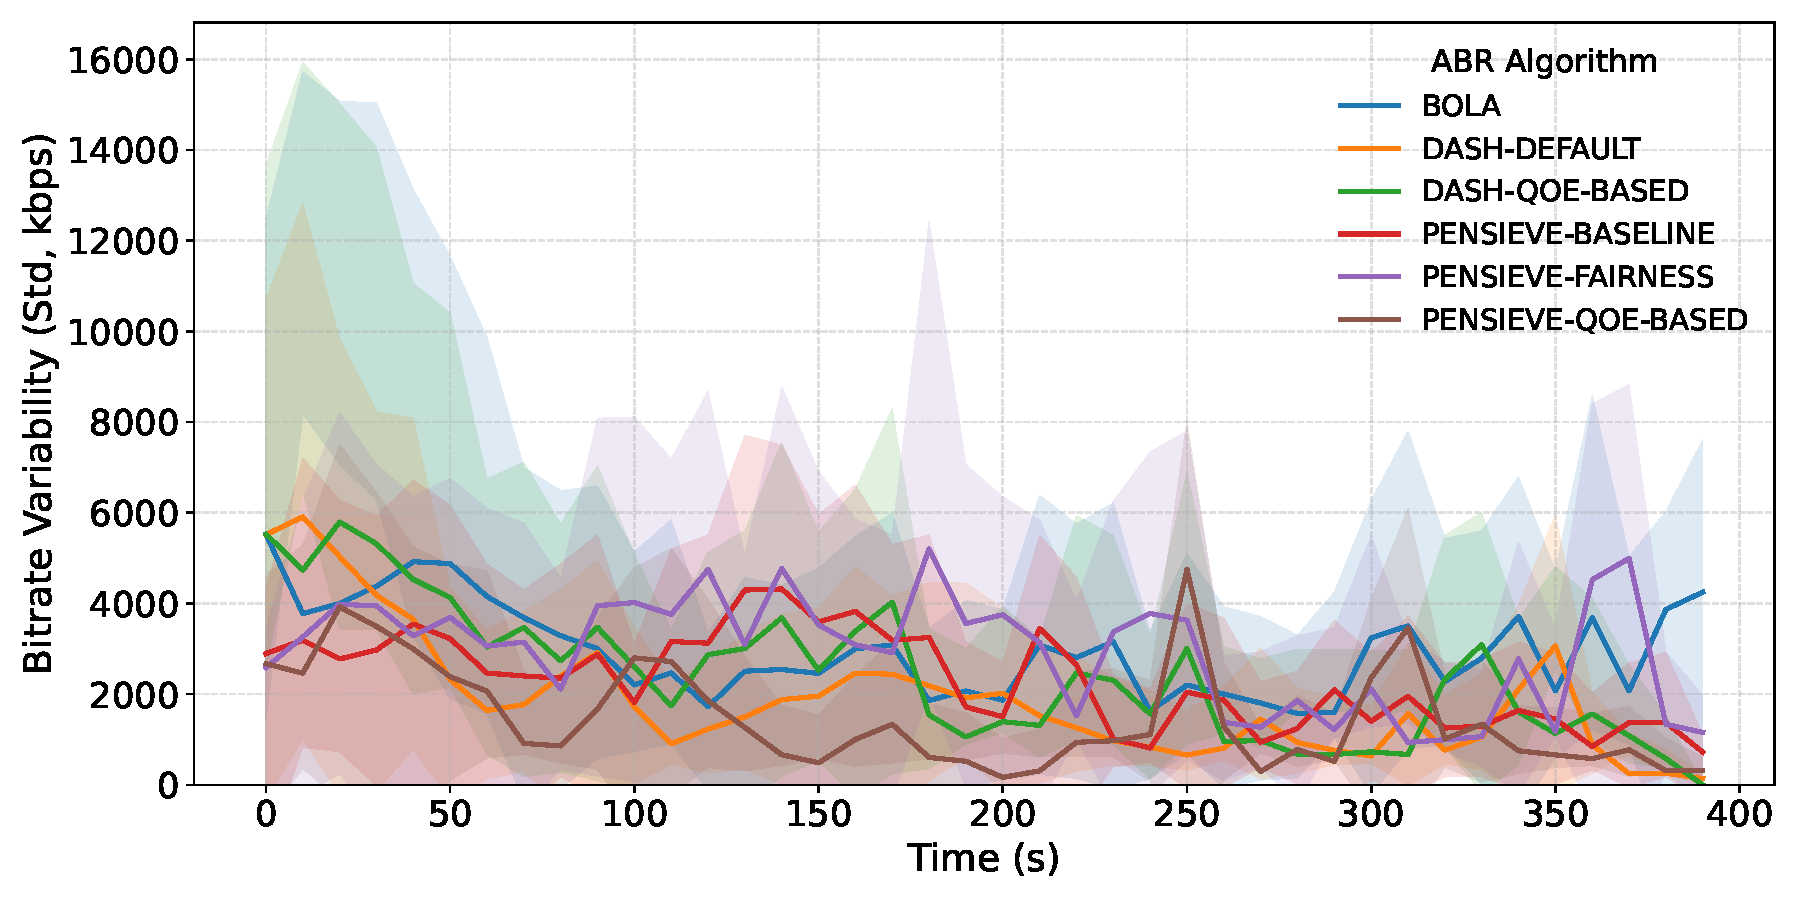
\includegraphics[width=0.98\linewidth,height=4.6cm,keepaspectratio=false]{images/p6-f4-network-variability-impact-3.pdf}
                \caption{Bitrate standard deviation timeline.}
                \label{fig:network_variability_exp3}
            \end{subfigure}
            \caption{Impact of adaptation logic and network variability on fairness metrics and bitrate distribution.}
            \label{fig:metrics_and_variability}
            \vspace{-0.3cm}
        \end{figure*}

    \subsection{Fairness Metric Behavior Across Adaptation Strategies}
    
        \vi{The analysis reveals that different ABR strategies exhibit distinct fairness profiles depending on the metric considered. Metrics capturing distributional aspects of user experience, such as QoE Fairness Score (QFS), often favor strategies that prioritize stable QoE exposure, whereas metrics related to resource allocation, such as Bitrate Fairness Index (BFI), may highlight different adaptation behaviors. This divergence indicates that fairness improvements observed under one metric may coexist with degradation according to another, reinforcing the need for a multi-metric evaluation perspective.}

        \vi{Figure~\ref{fig:fairness_metrics_exp3} illustrates this behavior under multi-client conditions. While most ABR strategies achieve consistently high QoE Fairness Score (QFS) values (typically above $\approx 0.9$), substantial disparities emerge when temporal fairness (TF-QoE) and bitrate distribution fairness (BFI) are considered. In particular, TF-QoE exhibits noticeable variation across adaptation strategies, whereas BFI shows pronounced degradation for algorithms that prioritize individual QoE maximization, with values dropping to the $0.7$–$0.8$ range in some cases. These results indicate that strategies maintaining stable QoE exposure across users do not necessarily ensure equitable bitrate allocation, especially under heterogeneous network conditions. Consequently, single-metric fairness evaluation may obscure relevant trade-offs, reinforcing the need for a multi-dimensional fairness analysis in adaptive streaming systems.}


    \subsection{Multi-Metric Fairness Interaction}

        \vi{Figure~\ref{fig:fairness_multimetric_interaction_exp3} analyzes the interaction between different fairness metrics under multi-client conditions using Spearman correlation analysis. The results reveal a strong positive correlation between TF-QoE and QoE Fairness Score (QFS) ($\rho \approx 0.94$), indicating that both metrics capture closely aligned aspects of perceived user experience fairness. In contrast, pronounced negative correlations are observed between QoE-oriented fairness metrics and bitrate distribution fairness. Specifically, QFS exhibits a strong negative correlation with the Bitrate Fairness Index (BFI) ($\rho \approx -0.77$), while TF-QoE shows a moderate negative correlation with BFI ($\rho = -0.60$). This pattern indicates that improvements in perceived QoE fairness are often accompanied by increased imbalance in bitrate allocation among competing clients. Stability-Aware Fairness (SAF), in turn, presents only weak correlations with the remaining metrics (|$\rho$| $\leq 0.14$), suggesting that adaptation stability captures a largely orthogonal fairness dimension. Overall, these interactions demonstrate that fairness metrics do not evolve independently and may encode competing objectives, particularly in heterogeneous and congested environments. Consequently, aggregated or single-metric fairness evaluation may obscure competing objectives between fairness dimensions.}

        
        \begin{figure*}[t]
            \centering
            \begin{subfigure}[b]{0.49\textwidth}
                \centering
                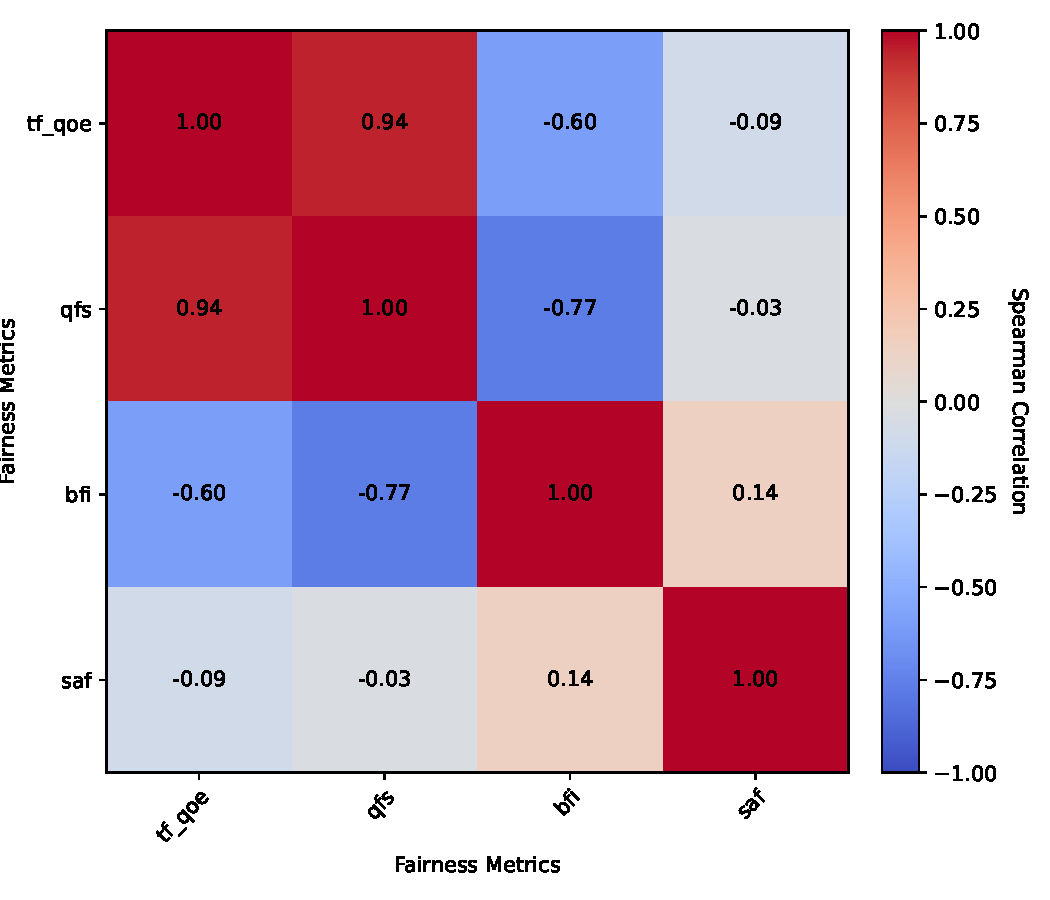
\includegraphics[width=0.98\linewidth,height=4.6cm,keepaspectratio=false]{images/P6-F2-multimetric-interaction-3.pdf}
                \caption{Spearman correlation heatmap.}
                \label{fig:fairness_multimetric_interaction_exp3}
            \end{subfigure}
            \hfill
            \begin{subfigure}[b]{0.49\textwidth}
                \centering
                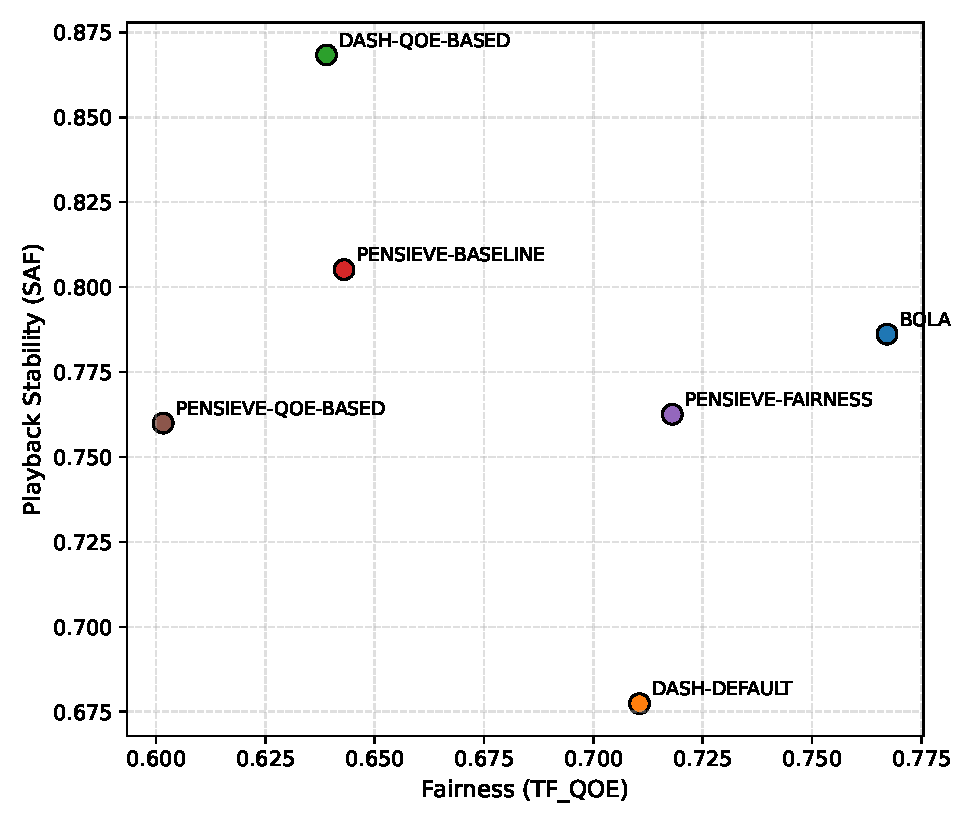
\includegraphics[width=0.98\linewidth,height=4.6cm,keepaspectratio=false]{images/P6-F3-fairness_stability_exp3_tf_qoe.pdf}
                \caption{SAF vs. TF-QoE interaction space.}
                \label{fig:fairness_stability_exp3}
            \end{subfigure}
            \caption{Interaction and trade-offs among fairness metrics and playback stability under multi-client conditions.}
            \label{fig:combined_interactions}
            \vspace{-0.3cm}
        \end{figure*}

    \subsection{Trade-offs Between Fairness and QoE Stability}

        \vi{A recurring pattern observed across scenarios is the interaction between fairness outcomes and QoE stability indicators, such as quality oscillations and rebuffering behavior. Figure~\ref{fig:fairness_stability_exp3} illustrates this interaction by jointly analyzing temporal fairness (TF-QoE) and playback stability (SAF) under multi-client conditions. The results show that adaptation strategies occupy distinct regions of the fairness–stability space, indicating that improvements along one dimension do not necessarily translate into gains along the other. Adaptation strategies that aggressively react to short-term throughput variations may improve fairness-related metrics but often at the cost of increased playback instability. As illustrated in Figure~\ref{fig:fairness_stability_exp3}, DASH-DEFAULT achieves moderate temporal fairness (TF-QoE $\approx 0.71$) but exhibits the lowest playback stability among the evaluated strategies (SAF $\approx 0.68$). In contrast, DASH-QoE-BASED prioritizes stability, reaching the highest SAF value (SAF $\approx 0.87$), while operating at lower temporal fairness levels (TF-QoE $\approx 0.64$). RL-based strategies occupy intermediate regions of the fairness–stability space. For instance, PENSIEVE-FAIRNESS improves temporal fairness relative to the baseline (TF-QoE $\approx 0.72$) while maintaining moderate stability (SAF $\approx 0.76$), whereas BOLA simultaneously achieves high fairness and stability (TF-QoE $\approx 0.77$, SAF $\approx 0.79$). These results confirm that fairness and stability objectives are not always aligned and that their trade-offs become more pronounced under heterogeneous and variable network conditions.}

        
    
    \subsection{Impact of Network Variability on Fairness Trade-offs}

        \vi{Network variability acts as a catalyst for fairness degradation, specifically by triggering asymmetric adaptation cycles across competing players. Figure~\ref{fig:network_variability_exp3} illustrates this behavior by plotting the standard deviation of selected bitrates across the fleet of 10 clients over time under the Verizon-LTE trace. 

        A walk-through of the timeline in Figure~\ref{fig:network_variability_exp3} reveals distinct operational phases. During the initial period of stable high bandwidth (first 25 seconds), the standard deviation remains very low ($\approx 2$~Mbps), indicating that all clients converge to similar high-quality representation levels. However, during throughput dips (e.g., around the 40s mark), reactive strategies exhibit a ``tactical panic'' where standard deviation spikes sharply to over 10~Mbps. This spike indicates that while the shared bottleneck capacity is equally reduced, the rate and timing of quality downswitching varies significantly across clients due to differences in individual buffer pressure.

        Furthermore, as the network stabilizes after the 80s mark, we observe a prolonged recovery period where the standard deviation remains persistently high ($\approx 8$~Mbps) for nearly 20 seconds. This slow convergence is driven by the ``recovery lag'' phenomenon. While the standard deviation plot shows the aggregate divergence, a micro-level analysis of individual client logs (e.g., Client 1 vs Client 8) reveals the underlying cause: Client 1 aggressively recovers to 2160p within 5 seconds of network restoration, whereas Client 8 remains ``locked'' at 360p/720p for up to 20 additional seconds to replenish its depleted buffer. This behavioral heterogeneity creates a persistent quality gap that aggregate, session-based metrics like JFI or QFS completely obscure, proving that recovery lag is a critical structural unfairness in decentralized ABR logic.}

    \subsection{Design Implications and Evaluation Scale}
        \vi{Our results suggest that achieving comprehensive fairness requires moving beyond individual bitrate maximization. We propose three actionable design shifts:
        \begin{itemize}[leftmargin=*, noitemsep, topsep=2pt, parsep=0pt]
            \item \textbf{Inter-Client Stability Constraints}: ABR controllers should incorporate the variance of switch counts $\sigma(S)$ into their objective functions. Designers should penalize strategies where specific users suffer disproportionate quality oscillations compared to the fleet average (SAF-aware control).
            \item \textbf{Synchronized Recovery Windows}: To mitigate the TF-QoE ``recovery lag,'' edge-assisted controllers should utilize cross-client synchronization to coordinate quality upswitches, preventing a subset of clients from monopolizing throughput during bandwidth recovery.
            \item \textbf{Asymmetric Reward Penalties}: In cellular-dominant environments, fairness-aware RL reward functions ($R$) should prioritize the standard deviation of perceived QoE over the session average ($\bar{Q}$), explicitly treating fairness as a stability-linked temporal dimension.
        \end{itemize}
        
        Single-metric optimization is structurally insufficient, and multi-dimensional evaluation is essential. A critical aspect of our evaluation is the balance between scale and architectural fidelity. While simulators (e.g., ns-3) can handle hundreds of agents, they abstract away the system-level overheads of real players. Our choice of 10 concurrent clients, each running a full Chromium instance via Selenium and a high-fidelity DASH.js player, ensures that our findings capture real-world resource contention (CPU/Memory cycles) that is absent in simulation. These implementation-heavy dynamics are essential for characterizing the ``tactical panic'' and ``recovery lag'' phenomena. For larger scales (50+ users), our analytical framework suggests that edge-assisted coordination becomes mandatory to mitigate the resource-heavy penalties of decentralized adaptation~\cite{alsader2025qoe}.}

\section{Conclusion and Future Work \label{sec:Conclusion and Future Work}}
    \vi{This study demonstrates that fairness trade-offs are structural properties of multi-client adaptive streaming systems, rather than anomalies of specific algorithms. Through a multi-metric observational analysis, we show that fairness is inherently multi-dimensional and cannot be adequately captured by single or aggregated indicators. Different ABR strategies occupy distinct regions of the fairness--stability space, reflecting structural trade-offs between responsiveness and conservatism under shared conditions. Our results reveal that network variability acts as a trade-off amplifier, exposing latent objective conflicts that remain obscured under stable scenarios. Rather than identifying a universally optimal strategy, this work emphasizes the need for structured, multi-dimensional evaluation frameworks that account for interacting metrics and network dynamics. Future work will investigate how these analytical insights can inform the design of edge-assisted, multi-objective learning strategies and coordinate recovery windows to balance competing fairness dimensions in next-generation 5G-Advanced and 6G environments.}


% \section*{Acknowledgment}
%     \scriptsize
%     This work was financed in part by the Fundação de Amparo à Pesquisa e Inovação do Estado de Santa Catarina (FAPESC) - Edital 24/2022 and the Federal Institute of Santa Catarina (IFSC). We also would like to thank the National Council for Scientific and Technological Development (CNPq) and the Federal University of Santa Catarina (UFSC) for partially supporting this study. Additionally, this article was edited for clarity and language improvement using ChatGPT, an AI-based language model.


\def\IEEEbibitemsep{0pt}
{\footnotesize
\bibliography{references}
\bibliographystyle{IEEEtran}
}


\end{document}

